\documentclass{article}
\usepackage[utf8]{inputenc}
\usepackage[T1]{fontenc}
\usepackage{tikz}
\usepackage{xcolor}

\begin{document}

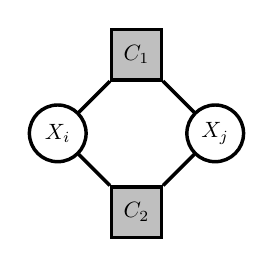
\begin{tikzpicture}[sq/.style={rectangle, scale=0.8, draw, fill=black!25, minimum size=0.8cm, inner sep=0pt},
c/.style={circle, scale=0.8, draw, minimum size=0.9cm, inner sep=0pt},
line width=1.25pt]

\node (0) [sq] at (0,1){$C_1$};
\node (1) [sq] at (0,-1){$C_2$};
\node (2) [c] at (-1,0){$X_i$};
\node (3) [c] at (1,0){$X_j$};
\draw[] (3) -- (0) -- (2) -- (1) -- (3);
\end{tikzpicture}

\end{document}